\documentclass[conference]{IEEEtran}
\IEEEoverridecommandlockouts
% The preceding line is only needed to identify funding in the first footnote. If that is unneeded, please comment it out.
\usepackage{cite}
\usepackage{amsmath,amssymb,amsfonts}
\usepackage{algorithmic}
\usepackage{graphicx}
\usepackage{listings}
\usepackage{textcomp}
\usepackage{xcolor}
\def\BibTeX{{\rm B\kern-.05em{\sc i\kern-.025em b}\kern-.08em
    T\kern-.1667em\lower.7ex\hbox{E}\kern-.125emX}}
\begin{document}

\title{Implementation and Evaluation of Differential Evolution Algorithm on CPU and GPU by using CUDA\\
% {\footnotesize \textsuperscript{*}Note: Sub-titles are not captured in Xplore and should not be used}
}

\author{\IEEEauthorblockN{Ali Khudiyev}
\IEEEauthorblockA{\textit{Data Science and Artificial Intelligence} \\
\textit{French-Azerbaijani University}\\
Baku, Azerbaijan \\
ali.khudiyev@ufaz.az}
}

\maketitle

\begin{abstract}
	Differential Evolution (DE) is one of the promising algorithms that is used for various optimization problems. It has a huge potential to be run on Graphics Processing Units (GPUs)
	since the algorithm uses single set of independent instructions(i.e., mutation, crossover, selection) on multiple data elements(i.e., vectors). In this paper, sequential version 
	of DEA is briefly discussed and massively parallel version is developed and evaluated to compare and understand the trade-offs between the different versions and hyperparameters of 
	the algorithm. Specific implmentation details such as algorithm architecture and optimization for CPU and GPU are discussed after introducing DE algorithm. Experiments are carried 
	on several times with the algorithm termination criteria of maximum number of objective function evaluations and statistical data are presented for the carried experiments.
	Results are discussed in terms of the presented statistical data and finally, conclusions and potential improvements for future work have been proposed and discussed briefly.
\end{abstract}

\begin{IEEEkeywords}
	Metaheuristics, Optimization, Differential Evolution, CPU, GPU, CUDA
\end{IEEEkeywords}

\section{Introduction}
Differential Evolution is one of the many metaheuristics used for various optimization problems. Main goal of the algorithm is to find global minimum of a given $n$-dimensional function by performing 
3 operations on the randomly initialized list of points or population. Different versions of DEs have been developed and widely used because of their promising results on the applied domains. However, 
the main problem that we may encounter while using such type of algorithms, is that the algorithm may get stuck in a local minimum, in other words, we have to avoid premature convergence in order to 
get the global minimum. In addition to that, each DE algorithm has some hyperparameters such as population size, crossover and mutation rates, number of generations which have to be tuned for each 
problem to be able to obtain the best results. However, DEA is very handy and flexible for various number of optimization problems since it has no assumptions or strict constraints for the problem 
it is applied to. Another benefit of using differential evolution comes from its nature; the algorithm is highly parallelizable as the performed operations are independent.

Implemention of sequential DEA on a CPU benefits the high speed of single core floating point calculations, however, true nature of the algorithm is not exploited due to the lack of parallelism. 
For the latter purpose, one could utilize GPGPUs (General Purpose Graphics Processing Units) that have many cores compared to CPUs. Using GPUs efficiently is also tricky due to several reasons shown below.

\begin{enumerate}
	\item Limited memory capcity and memory bandwidth
	\item Optimal utilization of shared and global memory
	\item Optimal schedule for limited number of SPs
\end{enumerate}

GPUs have memory components with many streaming processors that enable hardware/software parallelism. The common parallelism exploited by such GPUs are by performing Single Instruction Multiple Data (SIMD) 
operations. Such instructions are needed when there are potentially vast amount of data elements that need to go through same instruction execution pipeline. Obvious example of such computation paradigm is 
video games and graphics rendering. Two types of memory are common on GPUs: \textit{global} and \textit{shared}. Global memory is accessible for all processing units with low bandwidth and high capacity 
whereas shared memory is only accessible to subset of them with high bandwidth and low capacity. Shared memory according to NVIDIA developer blog \cite{b2}, is even faster than the local memory and the 
shared memory latency is roughly 100x lower than uncached global memory latency provided that there are no bank conflicts between the threads. Scheduling SPs (Streaming Processors) is also necessary in 
order to improve device utilization and gain potential run-time performance.

Graphics rendering or video games are not the only type of applications that may benefit from parallelism, in fact, what all GPUs do is vast amount of number crunching which can be handy for some scientific 
computations. However, we cannot just tell GPUs what to do without any specification or application programming interface (API). In previous years, OpenGL was the only option to write and execute 
programs on GPUs, but it was hard to use for scientific work since all the specification was built on pixel rendering pipeline that went through several stages(i.e., vertex, fragment, tesselation, 
geometry shaders). So, to do a scientific work on GPUs, one would need to transform the scientific calculations to some pixel-level calculations. Later on, NVIDIA developed Compute Unified Device 
Architecture (CUDA) which enabled programmers to execute instructions on GPUs more easily in a programmer-friendly way. 

\subsection{CUDA}

\begin{figure}[h]
	\centering
	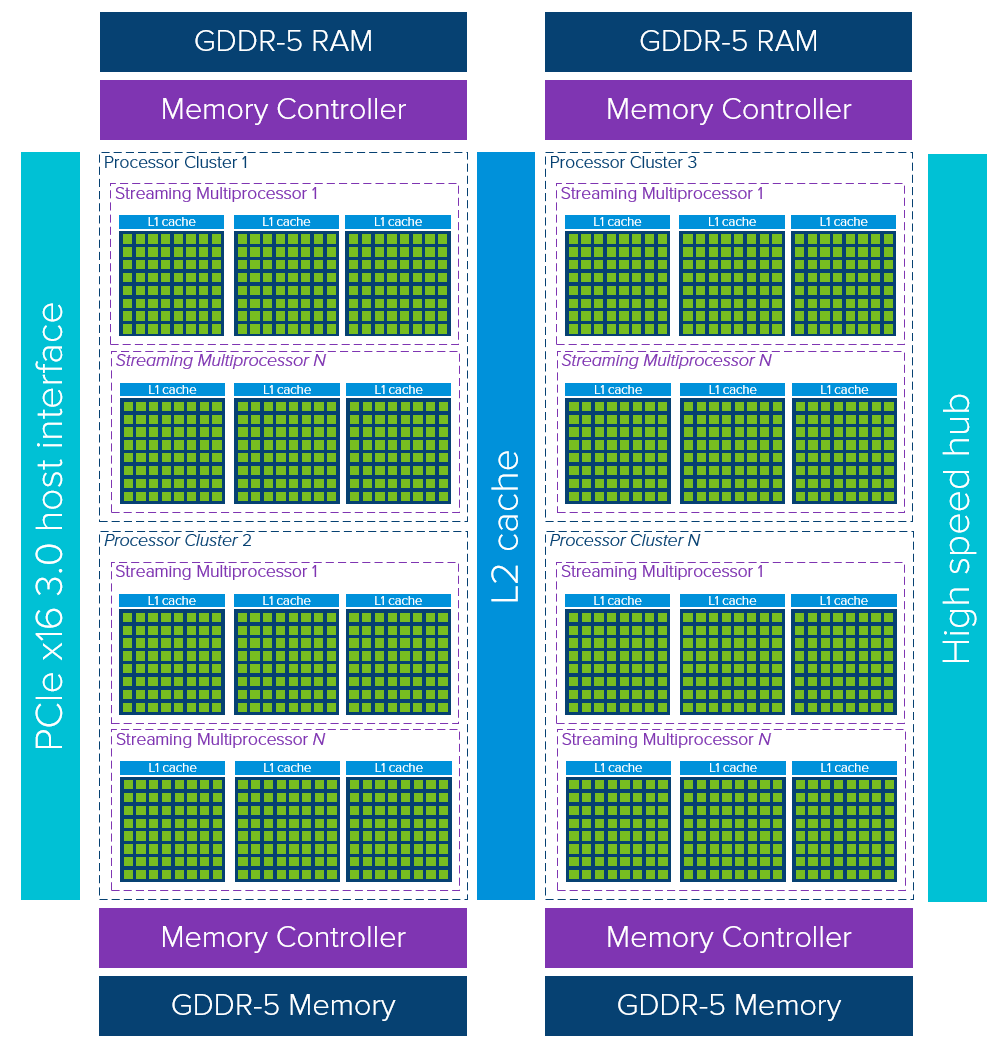
\includegraphics[width=0.75\linewidth]{img/gpu-architecture.png}
	\caption{GPU architecture}
	\label{fig:gpu_arch}
\end{figure}

Figure \ref{fig:gpu_arch} \cite{b1} illustrates common GPU architecture that has several processor clusters each of which contains several 
streaming multiprocessors. A multiprocessor consists of several streaming processors with many cores which have a shared L2 cache. Each streaming processor may also contain an L1 cache with higher 
memory bandwidth. There is also a memory controller that enables processors to utilize the global main memory of the card which has more capacity with lower bandwidth.

To execute a program on a GPU by using CUDA, we need to use C-like language called CUDA-C and there are 4 general steps to follow: \textit{copy data from main memory to GPU memory}, 
\textit{send instructions from CPU to GPU}, \textit{execution on GPU}, \textit{copy data back from GPU memory to main memory}. These 4 steps are easy to follow and enable programmers 
to write their custom codes which are executed on GPU side. CUDA-C has keywords \textbf{\lstinline{__global__}} and \textbf{\lstinline{__device__}} that can be used to indicate that 
if a function executed by GPU is callable by the host or the device respectively. The functions defined with the \textbf{\lstinline{__global__}} keyword are also called \textbf{kernels}.

\section{Sequential DE}
Implementation of Differential Evolution algorithm on CPUs is straight forward for many educational cases. However, it requires relatively more knowledge of underlying working principles of CPU/GPUs and 
their architectures to be able to use all of what the modern technology offers in terms of power and efficiency. There are many implementation principles such as pass-by-reference 
(to reduce memory operations, instead of pass-by-value), dynamic programming (DP) (to reduce memory operations), single instruction multiple data (SIMD) operations 
(to reduce computation time, instead of SISD) and so on. In this project, some of the underlying best practices are used while implementing the sequential differential evolution algoritm. 

\subsection{Overview of DEA}
As other metaheuristics, DE tries to minimize or maximize the objective function. To maximize a given objective function $F$, we could transform it to $-F$ and try to minimize this function 
instead, and we can even try to approximate to particular output value of the function by transforming it into $(F-f_\text{bias})^2$ where $f_\text{bias}$ is the approximated point. 
There are 3 steps which the algorithm uses to evolve a generation of individuals: \textit{mutation}, \textit{crossover} and \textit{selection}. Each of these steps are discussed briefly in this section.

\subsubsection{Mutation}
Mutation operation is usually the first operation executed and it introduces a concept of diversity in differential evolution algorithms. There are many mutation operators that have been discovered 
and used for many problems, however, the best mutation operator is still subject to the given problem. For example, classic mutation operator would be moving an individual according to the direction 
obtained by the subtraction between two different randomly chosen individuals on some dimensional space. This version of mutation operator is called DE/rand/1 and it is widely known operation.
However, there are other methods such as DE/best/1, DE/current-to-best/1, DE/current-to-rand/1, DE/rand-to-best that work with slightly different modifications. The mutation operator implemented 
in this project is \textit{unified mutation strategy} \cite{b3} which is shown below.

\begin{equation}
	\begin{split}
		v_i = &x_i + F_1 (\bar{x}_b - \bar{x}_i) + F_2 (\bar{x}_{r_1} - \bar{x}_i) \\
			& + F_3 (\bar{x}_{r_2} - \bar{x}_{r_3}) + F_4 (\bar{x}_{r_2} - \bar{x}_{r_3})
	\end{split}
	\label{eq:mutation_operation}
\end{equation}

where $F_1$, $F_2$, $F_3$ and $F_4$ are four potentially adaptively adjustable parameters, $r_i$ is a randomly generated index $i$, $x_b$ is an individual with the best fitness value among the whole population. 
Assigning each scaling parameter $F_i$ to 0 produces different versions of previously mentioned mutation strategies. For this project, $F_1 = F_2 = 0.25$ and $F_3 = F_4 = 0.2$ are set statically.

\subsubsection{Crossover}
Crossover operation is used to mix two individuals together in terms of their individual coordinates in some high dimensional space.

\begin{equation}
	u_{ij} = 
	\begin{cases}
		v_{ij}, &\text{if rand}_j \leq \text{CR or } j = \text{mbr} \\
		x_{ij}, &\text{otherwise}
	\end{cases}
	\label{eq:crossover_operation}
\end{equation}

where \lstinline{CR} is the crossover rate and \lstinline{mbr} is the last index of an individual. For this project, $\text{CR} = 0.8$ is set statically.

\subsubsection{Selection}
Selection is the last operation that is implemented in order to obtain a new set of individuals. New generation is obtained by filtering out some individuals that have less fitness values compared to their 
children. At the end of each generation, we replace an individual with another individual, therefore, the number of individuals in any generation remains the same through the whole execution.

\begin{equation}
	x^{\prime}_i = 
	\begin{cases}
		u_i, &\text{if } f(u_i) < f(x_i) \\
		x_i, &\text{otherwise}
	\end{cases}
	\label{eq:selection_operation}
\end{equation}

where $f$ is the objective or cost function to be minimized.

\subsection{Sequential DE Architecture}
Although we could reduce computation complexity by using some of the best practices, such as using DP when evaluating cost functions, using arithmetic vector operations or reducing copy instructions by 
using pointers, there is a big limitation in terms of computation time since mutation, crossover and selection are performed per an individual one at a time. The architecture for the sequential 
DE is shown below to be able to compare later with the parallelized architecture.

\begin{figure}[h]
	\centering
	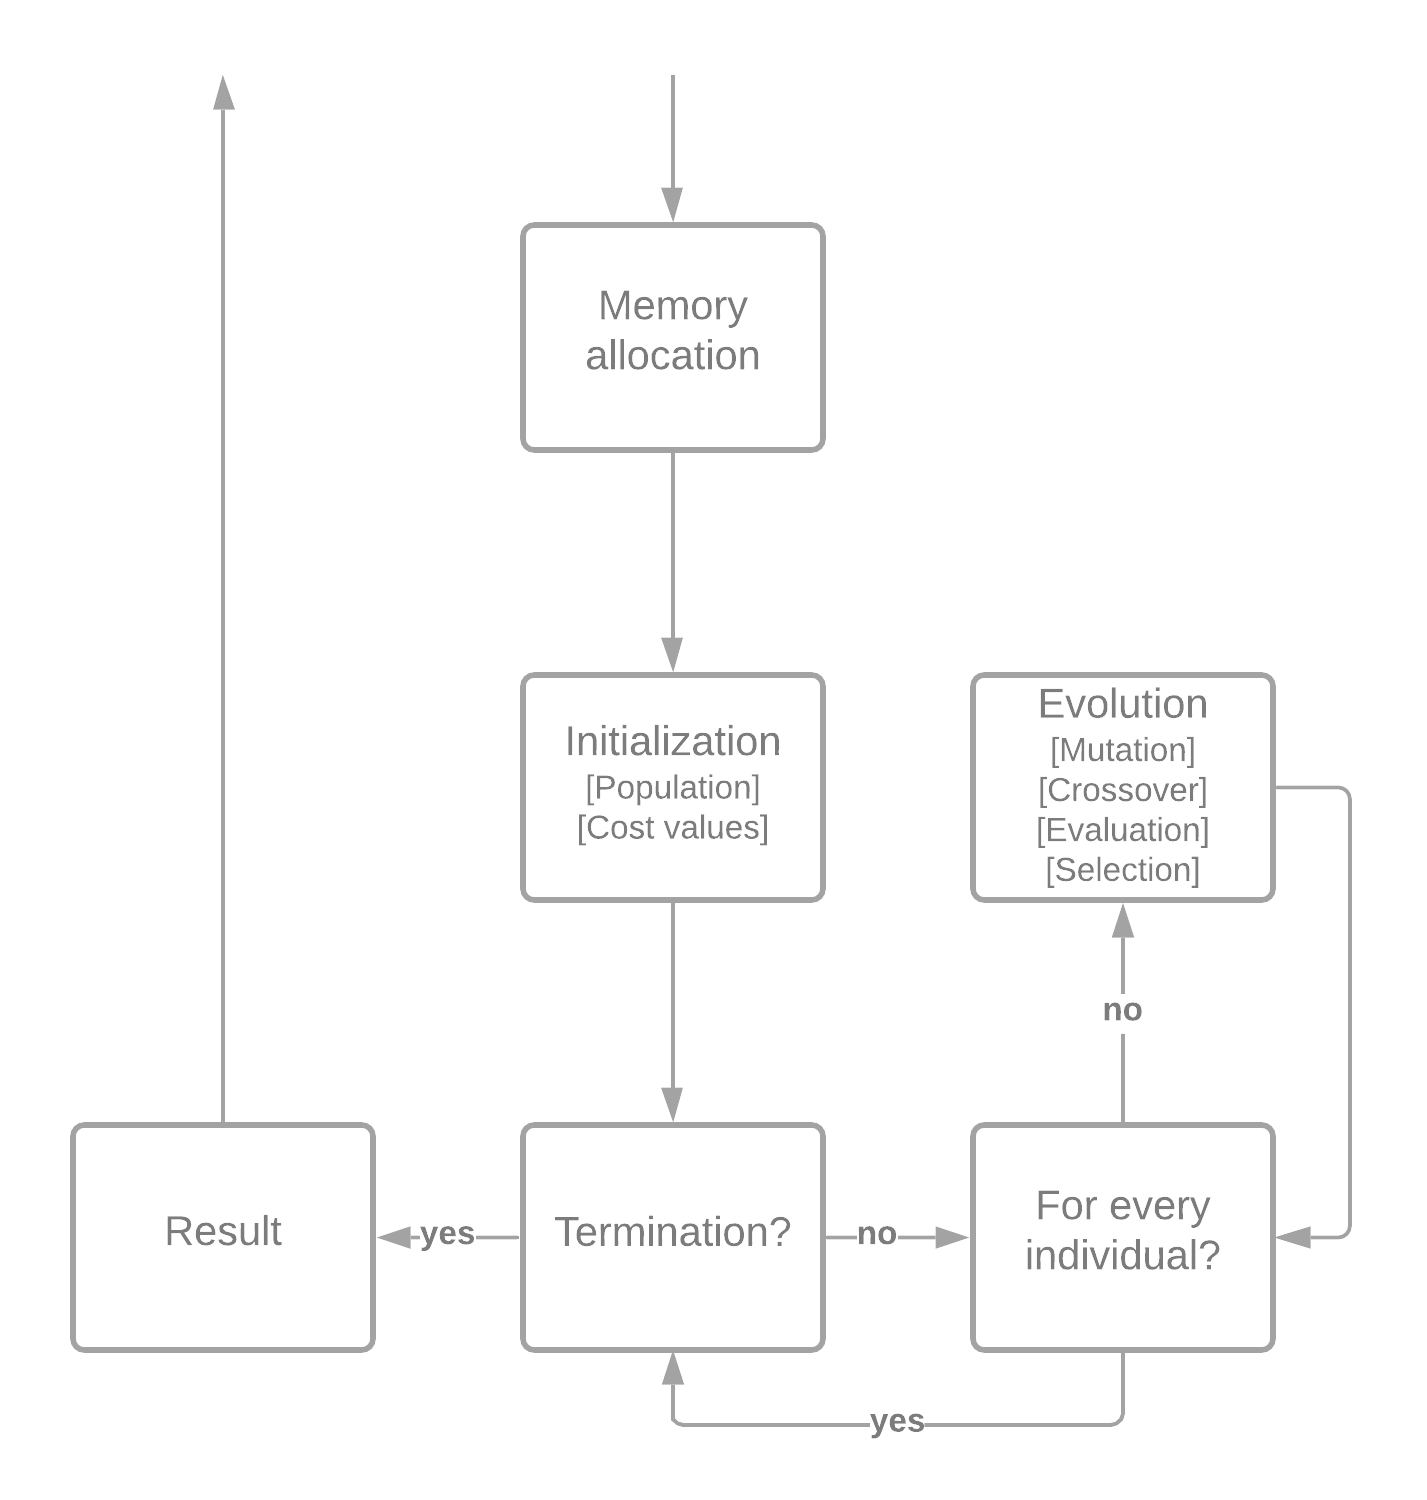
\includegraphics[width=0.75\linewidth]{img/seq_arch.png}
	\caption{Sequential DE Architecture}
	\label{fig:seq_arch}
\end{figure}

As shown in figure \ref{fig:seq_arch}, we begin by initilizing the population randomly after which the main loop starts executing untill the termination criteria is met. Inside each iteration, 
we develop another loop to perform MCES(mutation, crossover, evaluation, selection) for each individual of the population. The time needed to perform MCES for an individual accumulates inside 
the inner loop and since MCES are independent operations, there is a huge potential for this part of the program to be parallelized.

\section{Parallel DE with CUDA}
It is common to use GPUs to run different versions of DEA since they offer massively parallel environment that can overperform even CPUs with higher clock rates simply due to efficient utilization of 
same instructions on massive amount of data. In this paper, a simple CUDA-based implementation of the DEA is described by using its architecture and discussing the advantages, disadvantages and 
possible imporovements. The proposed CUDA-based implementation have been developed in a generic and user-friendly manner, meaning that one has flexibility over the algorithm by being capable of 
easily chaning population size, dimension of the objective functions(i.e., Rastrigin, Rosenbrock, Griewank and Sphere), crossover and mutation rates.

\subsection{Proposed architecture for GPU version of DEA}
The developed CUDA-based DE is one example implementation of the algorithm and it has a simple architecture which is shown in figure \ref{fig:mp_arch}. In the implementation, GPU calls 
are made once per generation and each operator described above are executed withing one kernel called \textit{evolutionKernel}. There are several limitations with this implmentation such as number 
of individuas within a population(\textit{popSize}), memory bandwith and memory allocation. GPU calls are made with the following parameters: $\textit{gridDim}=1$ and 
$\textit{blockDim}=\lceil \textit{popSize} / 32 \rceil * 32$. For potential performance boost, the number of threads are selected as powers of 2.

\begin{figure}[h]
	\centering
	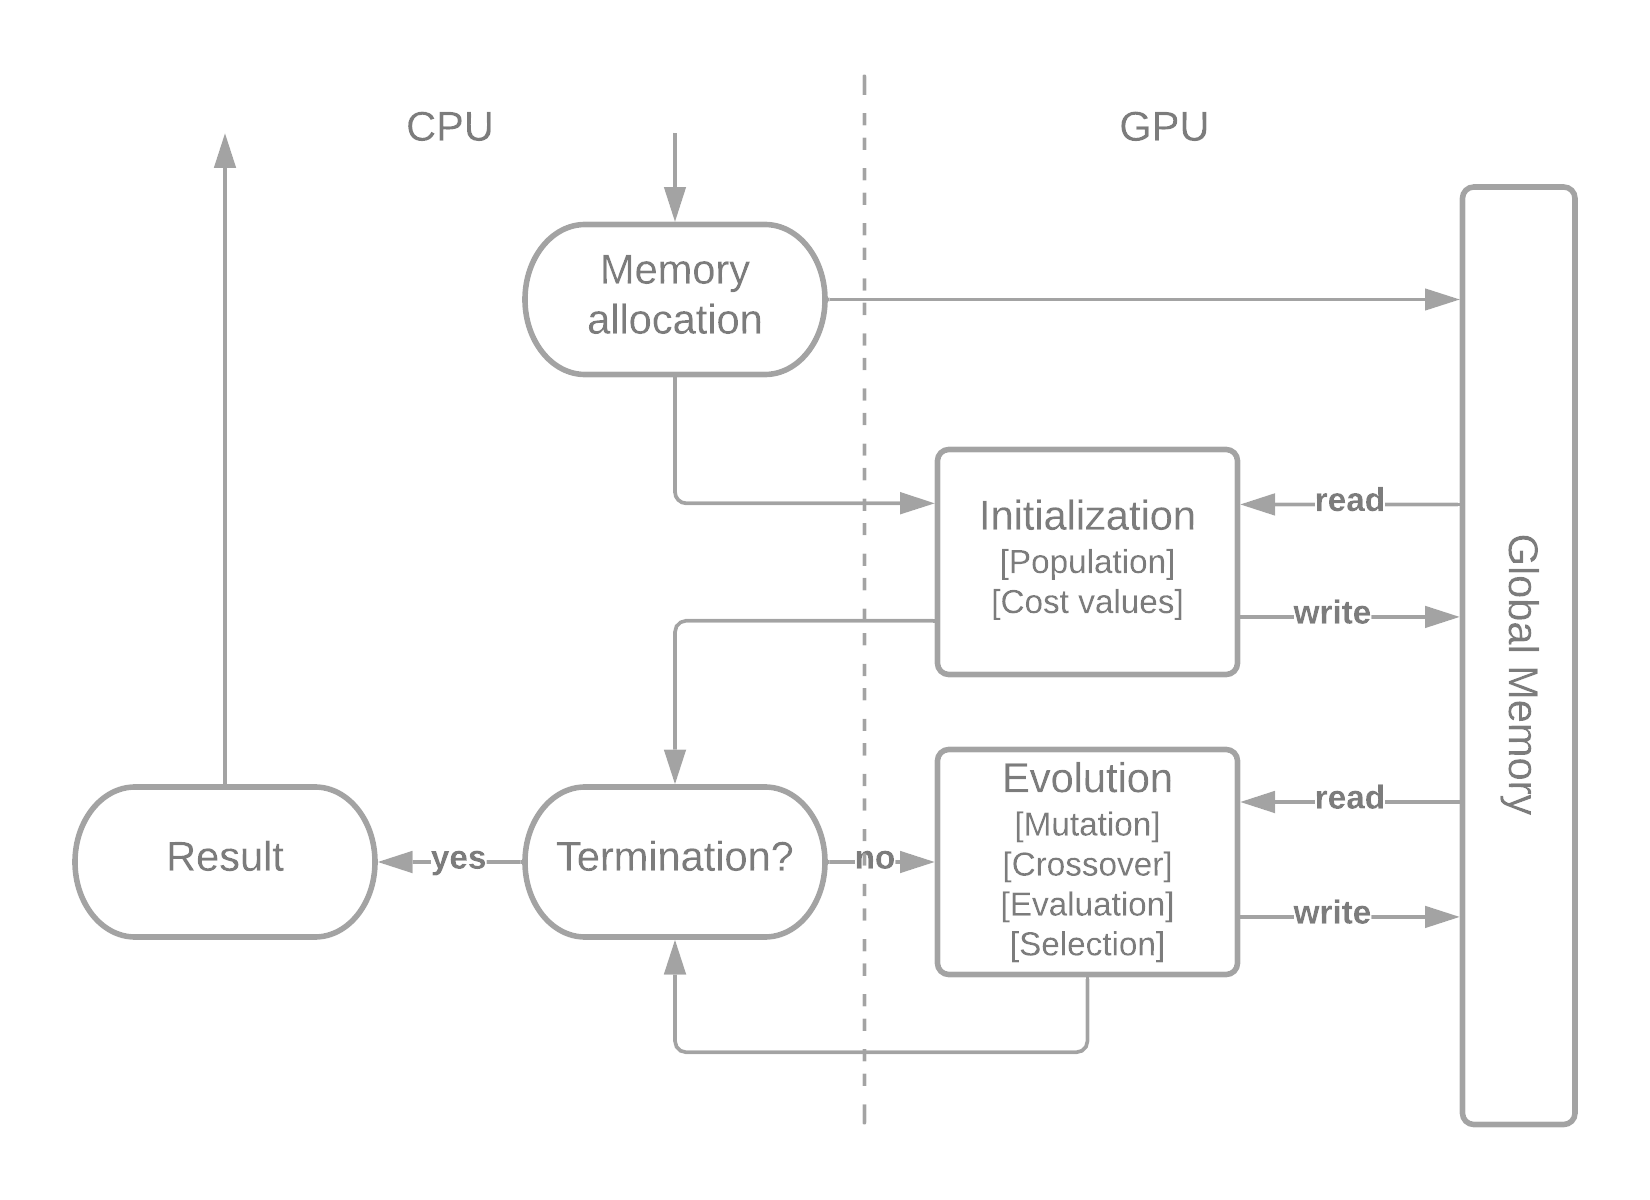
\includegraphics[width=0.75\linewidth]{img/arch.png}
	\caption{Massively Parallel DE Architecture}
	\label{fig:mp_arch}
\end{figure}

By comparing the figure shown above with the figure \ref{fig:seq_arch}, the differences are obvious - parallelized \textit{initialization of population and costs} and \textit{MCES} operations 
have been parallelized. The nested loop that is executed \textit{for every individual} in the sequential version is written in a massively parallel way. These two kernels uses some CUDA 
functions for random number generation and device or thread synchronization and they have been defined with \textbf{\lstinline{__global__}} keyword since they are called from the host and 
there are functions that are defined with \textbf{\lstinline{__device__}} keyword which are only callable by the GPU.

\begin{itemize}
	\item \textbf{Initalization} kernel - initilization of population by using predifined random states needed for \textbf{\lstinline{curand_uniform(state)}} function which generates a number in the 
		interval of $(0, 1]$ with the uniform distribution. After each thread initializes the corresponding individual, selected cost function is called on the individual and the output value is 
		stored in a device buffer for later use.
	\item \textbf{Evolution} kernel - radom index generation, best index selection, mutation, evaluation, crossover, selection are performed in this function. Random indices are compared with each other 
		to make sure that no same indices are used for MCES. Each thread representing a unique individual in the population compares its current cost value with the global minimum cost value and if the 
		cost value is less than the global one, the best individual's index and cost value are updated globally. Threads are synchronized with \textbf{\lstinline{__syncthreads()}} after this comparison 
		step to be able to obtain the best or near-to-best individual's index to be able to carry the unified mutation strategy. Device-generated random numbers are used to decide when to apply mutation 
		and crossover and evaluated cost values rewrite the host and device buffers which held the old costs.
\end{itemize}

\section{Experiments}
\subsection{Experimental Environment}
The environment for running CUDA-based DE algorithm was set up in \textit{Google Colab} with the installation of \textit{cuda-9.2} and GPU runtime type. Sequential version of the algorithm was executed in 
Mac with the \textit{Intel core i7 2.6-4.5Ghz} CPU. The experiments have been carried out for \textit{Rastigin}, \textit{Rosenbrock}, \textit{Griewank} and \textit{Sphere} functions with 
4 different population sizes(50, 100, 500, 1000), 3 dimensions(10, 50, 100), termination criteria of $10^4 * \text{dim}$ number of objective function evaluations and 25 benchmark runs for each objective function.

\begin{equation*}
	f_\text{sphere} = \sum_{i=1}^{i=D} z_i^2 + f_\text{bias}
	\label{func:sphere}
\end{equation*}

\begin{equation*}
	f_\text{rastrigin} = \sum_{i=1}^{i=D} (z_i^2 - 10\cos(2\pi z) + 10) + f_\text{bias}
	\label{func:rastrigin}
\end{equation*}

\begin{equation*}
	f_\text{rosenbrock} = \sum_{i=1}^{i=D-1} (100(z_i^2 - z_{i+1})^2 + (z_i - 1))^2 + f_\text{bias}
	\label{func:rosenbrock}
\end{equation*}

\begin{equation*}
	f_\text{griewank} = \sum_{i=1}^{i=D} \frac{z_i^2}{4000} + \prod_{i=1}^{D} \cos(\frac{z_i}{i}) + 1 + f_\text{bias} 
	\label{func:griewank}
\end{equation*}

where $z = x - o$ and $o = \bar{0}$, $f_\text{bias} = 0$.

\subsection{Results}
The figures \ref{fig:10d_popsize_time}-\ref{fig:100d_popsize_time} show the relation between run-time and population size for each benchmark function. It is obvious from the figures that as the population 
size increases, run-time decreases which is due to the decreasing number of generations which is calculated as shown below.

\begin{equation}
	\text{nbGen} = \frac{10^4 \cdot D}{\text{popSize}}
	\label{eq:nbgen}
\end{equation}

For each generation, the selected objective function is evaluated once per an individual and when the dimension($D$) is fixed to 10, 50, 100, we need to reduce the number of generations in order to comply 
with the termination criteria. Due to such restriction on the number of objective function evaluations, DEA runs with $200D$, $100D$, $20D$ and $10D$ generations respective to $50$, $100$, $500$, $1000$ 
population sizes.

\begin{figure}[h]
	\centering
	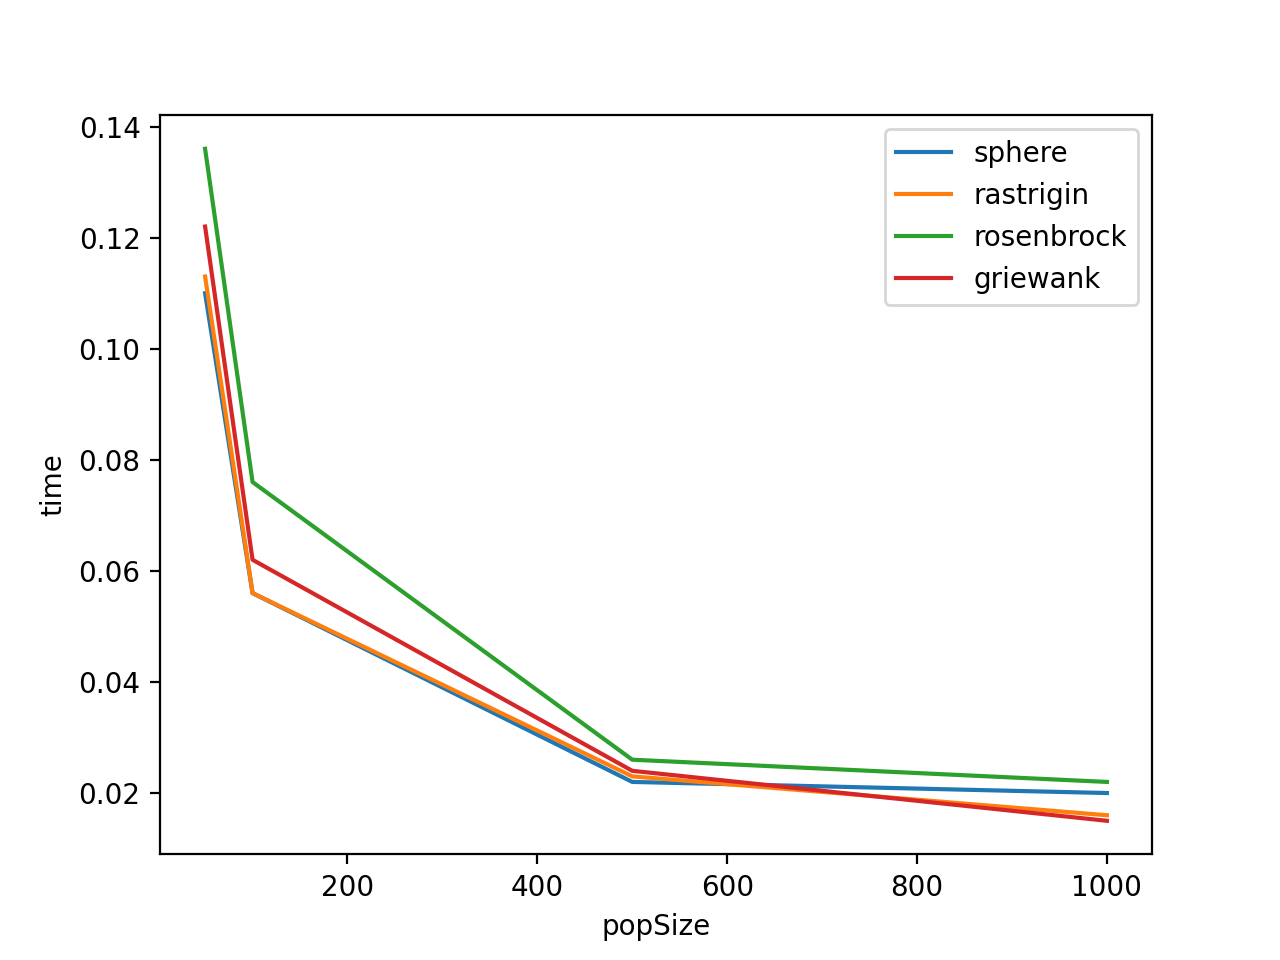
\includegraphics[width=0.75\linewidth]{img/10D_popSize_time.png}
	\caption{Time-population size for 10D functions}
	\label{fig:10d_popsize_time}
\end{figure}

\begin{figure}[h]
	\centering
	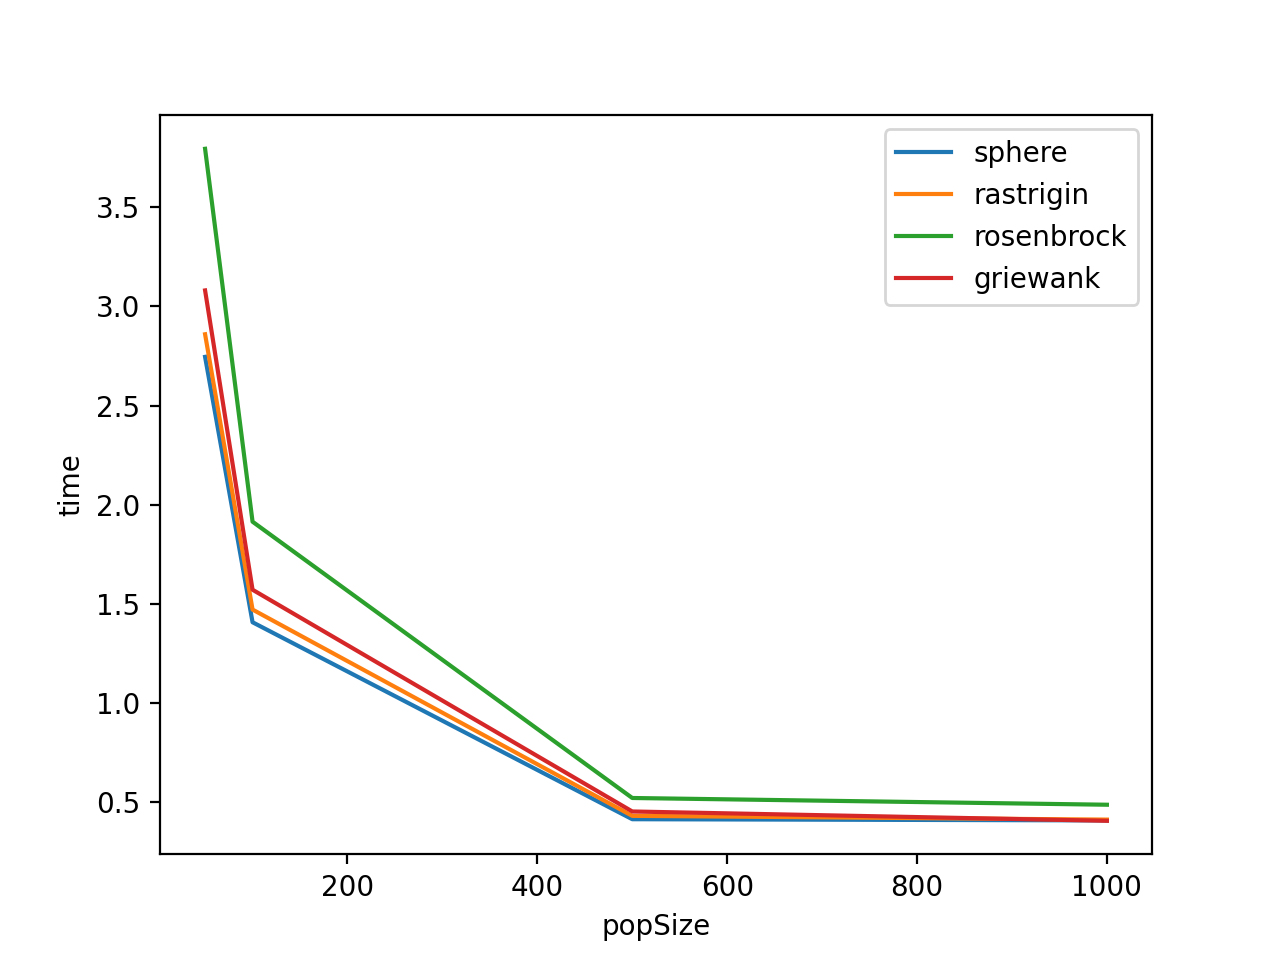
\includegraphics[width=0.75\linewidth]{img/50D_popSize_time.png}
	\caption{Time-population size for 50D functions}
	\label{fig:50d_popsize_time}
\end{figure}

\begin{figure}[h]
	\centering
	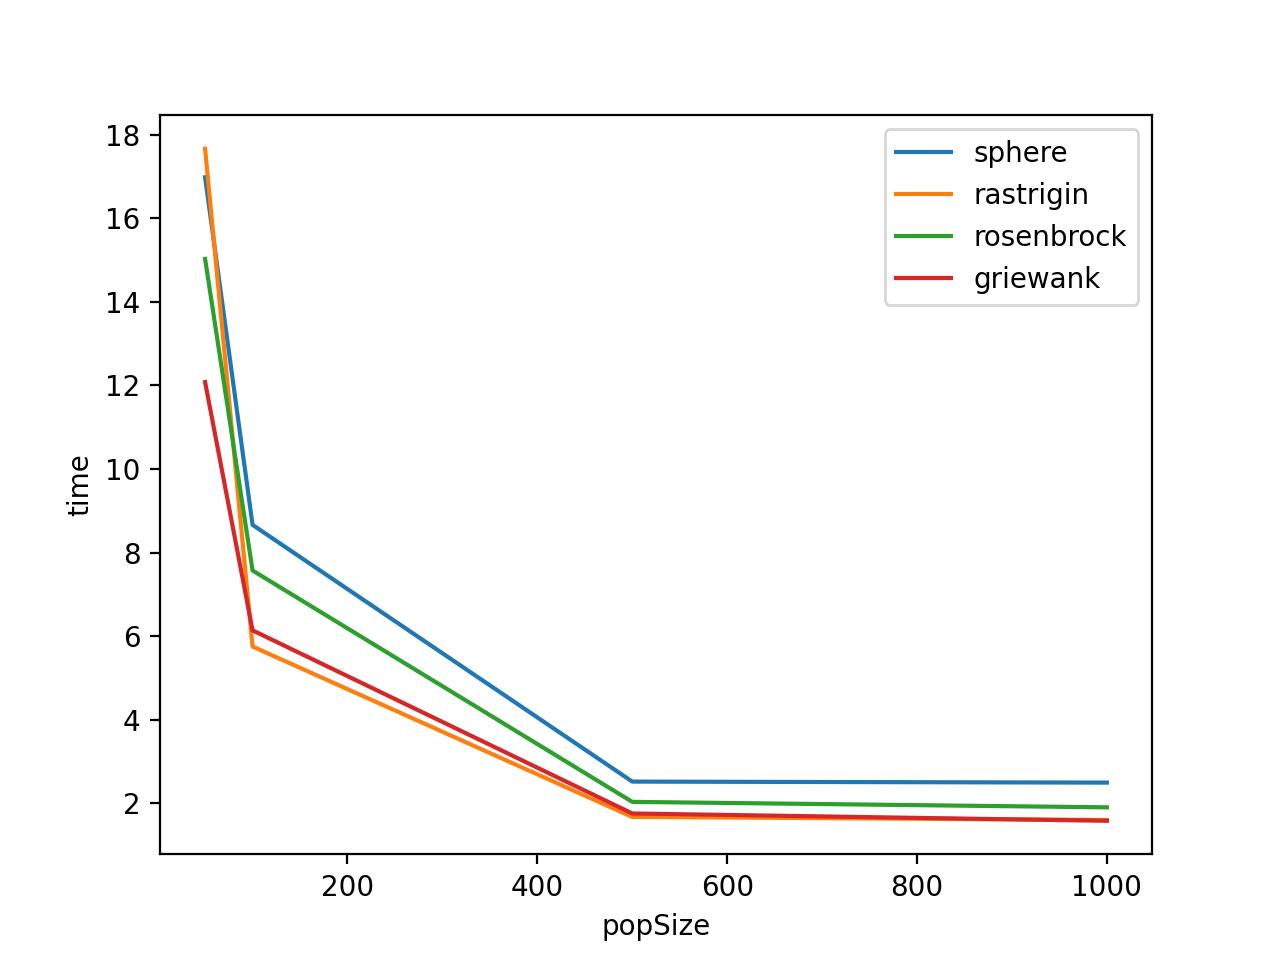
\includegraphics[width=0.75\linewidth]{img/100D_popSize_time.png}
	\caption{Time-population size for 100D functions}
	\label{fig:100d_popsize_time}
\end{figure}

The best cost values for each objective functions is shown with the bold fonts in the tables \ref{tab:benchmark}-\ref{tab:benchmark3}. As the number of individuals in a population increases, the quality 
of solutions decrease, and the number of individuals is inverse proportional to run-time of the algorithm. According to the tables, almost all the best solutions for any benchmark function has been 
achieved with 100 individuals with the exception of 50D Rosenbrock function for which the best solution was found with 50 individuals, however, the second best solution was found with 100 individuals 
with the absolute difference of $0.001$. The quality of the best obtained solutions gets better from Rosenbrock to Rastrigin, then to Griewank, and to Sphere function for which the solution was the best 
among all other benchmark functions in terms of the minimized cost value.

\begin{table}[h]
	\centering
	\begin{tabular}{|c|c|c|c|c|c|}
		\hline
		\textbf{Function} & & \textbf{P50} & \textbf{P100} & \textbf{P500} & \textbf{P1000} \\
		\hline
		Sphere 			& Mean & 0.000 & 0.000 & 0.000 & 0.201 \\
						& Std & 0.000 & 0.000 & 0.000 & 0.053 \\
						& Best & \textbf{0.000} & \textbf{0.000} & \textbf{0.000} & 0.101 \\
						& Time & 0.110 & 0.056 & 0.022 & 0.020 \\
		\hline
		Rastrigin 		& Mean & 0.000 & 0.000 & 0.190 & 3.110 \\
						& Std & 0.000 & 0.000 & 0.066 & 0.583 \\
						& Best & \textbf{0.000} & \textbf{0.000} & 0.110 & 1.626 \\
						& Time & 0.113 & 0.056 & 0.023 & 0.016 \\
		\hline
		Rosenbrock 		& Mean & 1.378 & 1.142 & 12.412 & 196.760 \\
						& Std & 3.385 & 1.546 & 5.386 & 52.778 \\
						& Best & 0.041 & \textbf{0.039} & 3.448 & 121.534 \\
						& Time & 0.136 & 0.076 & 0.026 & 0.022 \\
		\hline
		Griewank 		& Mean & 0.003 & 0.003 & 0.034 & 0.406 \\
						& Std & 0.001 & 0.001 & 0.010 & 0.099 \\
						& Best & \textbf{0.002} & \textbf{0.002} & 0.015 & 0.175 \\
						& Time & 0.122 & 0.062 & 0.024 & 0.015 \\
		\hline
	\end{tabular}
	\caption{D10}
	\label{tab:benchmark}
\end{table}

\begin{table}[h]
	\centering
	\begin{tabular}{|c|c|c|c|c|c|}
		\hline
		\textbf{Function} & & \textbf{P50} & \textbf{P100} & \textbf{P500} & \textbf{P1000} \\
		\hline
		Sphere 			& Mean & 0.000 & 0.000 & 0.002 & 11.377 \\
						& Std & 0.000 & 0.000 & 0.0003 & 1.925 \\
						& Best & \textbf{0.000} & \textbf{0.000} & 0.001 & 8.133 \\
						& Time & 2.746 & 1.408 & 0.415 & 0.409 \\
		\hline
		Rastrigin 		& Mean & 5.219 & 3.838 & 11.872 & 41.254 \\
						& Std & 1.036 & 1.158 & 0.852 & 2.275 \\
						& Best & 3.308 & \textbf{1.992} & 10.160 & 37.117 \\
						& Time & 2.860 & 1.472 & 0.432 & 0.413 \\
		\hline
		Rosenbrock 		& Mean & 6.855 & 1.015 & 120.791 & 18839.424 \\
						& Std & 6.396 & 0.898 & 18.013 & 4368.884 \\
						& Best & \textbf{0.090} & 0.091 & 82.676 & 8976.218 \\
						& Time & 3.795 & 1.915 & 0.522 & 0.488 \\
		\hline
		Griewank 		& Mean & 0.003 & 0.003 & 0.018 & 1.098 \\
						& Std & 0.0005 & 0.001 & 0.007 & 0.016 \\
						& Best & \textbf{0.002} & \textbf{0.002} & 0.010 & 1.056 \\
						& Time & 3.081 & 1.572 & 0.454 & 0.407 \\
		\hline
	\end{tabular}
	\caption{D50}
	\label{tab:benchmark2}
\end{table}

\begin{table}[h]
	\centering
	\begin{tabular}{|c|c|c|c|c|c|}
		\hline
		\textbf{Function} & & \textbf{P50} & \textbf{P100} & \textbf{P500} & \textbf{P1000} \\
		\hline
		Sphere 			& Mean & 0.000 & 0.000 & 0.008 & 43.662 \\
						& Std & 0.000 & 0.000 & 0.002 & 4.174 \\
						& Best & \textbf{0.000} & \textbf{0.000} & 0.005 & 34.027 \\
						& Time & 16.983 & 8.664 & 2.520 & 2.496 \\
		\hline
		Rastrigin 		& Mean & 13.934 & 10.851 & 31.111 & 101.171 \\
						& Std & 1.324 & 2.095 & 1.783 & 2.886 \\
						& Best & 10.995 & \textbf{6.074} & 28.335 & 95.523 \\
						& Time & 17.664 & 5.752 & 1.675 & 1.602 \\
		\hline
		Rosenbrock 		& Mean & 15.061 & 2.056 & 334.446 & 93407.289 \\
						& Std & 12.897 & 1.555 & 32.649 & 16300.186 \\
						& Best & 1.641 & \textbf{0.454} & 269.263 & 60801.457 \\
						& Time & 15.029 & 7.572 & 2.035 & 1.904 \\
		\hline
		Griewank 		& Mean & 0.004 & 0.003 & 0.025 & 1.394 \\
						& Std & 0.002 & 0.002 & 0.007 & 0.044 \\
						& Best & \textbf{0.002} & \textbf{0.002} & 0.016 & 1.303 \\
						& Time & 12.081 & 6.140 & 1.757 & 1.582 \\
		\hline
	\end{tabular}
	\caption{D100}
	\label{tab:benchmark3}
\end{table}

When comparing to the results obtained by $\text{cudaDE}_\text{i}$\cite{b4} developed by the people from INRIA Grenoble Rhone-Alpes and Nanyang Technological University, we can observe that they have 
similar decreasing run-time as the population size increases for a fixed dimension and they have also achieved the best results with 100 and 50 individuals. However, overall run-time of the DE algorithm 
described in this paper is slightly less than their run-time which is due to the different experimental envrionments. The results shown in this paper are run on Google Colab's GPU which has superior 
performance. The best results for Griewank function are achieved with the cost value of $0.002$ for any dimension in this project whereas $\text{cudaDE}_\text{i}$ obtained $0.000$ with 500 and 1000 
individuals for any dimension. The best results for Sphere function are of the same quality ($0.000$) and for the results obtained in this project are better or same for Rastrigin and Rosenbrock functions.

\section{Conclusion and Future work}
Sequential and massively parallel versions of DE algorithm have been developed and evaluated with 4 benchmark functions. Sequential DE algorithm consumes more run-time than that of the parallel version and 
it is obvious that how the algorithm with a parallel nature can benefit from massive parallelism that GPUs offer. Programming for NVIDIA's GPUs is also more straight forward now becaues of the CUDA toolkit 
which provides programmers with a C-like language to work with.

There are many possible improvements for the CUDA-based DE implementation described in this paper. Global versus shared memory utilization could be optimized for the future work in order to increase 
memory bandwith since currently it could be bottlenecked by large amount of data flow from/to global memory. Another potential performance gain could come from using modular devicde functions in GPU 
rather than using just a single evolution kernel.

\section{Acknowledgments}
In the development of this project, I thank authors of $\textit{cudaDE}_\textit{i}$ and \textit{unified mutation strategy} for sharing their works. In addition, the professor Lhassane Idoumghar gave me 
useful information and insights about some details and the related topics. In this alone journey with full of projects, he has given support for this project work.

\begin{thebibliography}{00}
\bibitem{b1} Exploring GPU Architecture. https://core.vmware.com/resource/exploring-gpu-architecture.
\bibitem{b2} NVIDIA Developer Blog. https://developer.nvidia.com/blog/using-shared-memory-cuda-cc/.
\bibitem{b3} Ji Qiang and C. Mitchell, ``A unified differential evolution algorithm for global optimization``.
\bibitem{b4} A. K. Qin, F. Raimondo, F. Forbes and Y. S. Ong, ``An improved CUDA-based implementation of differential evolution on GPU``.
\end{thebibliography}

\end{document}
